% !TeX root = ../tfg.tex
% !TeX encoding = utf8

\chapter{Resultados}

El trabajo ha conseguido cumplir algunos de sus objetivos: Se ha construido una librería en Scala que implementa la
paralelización del proceso de aprendizaje de redes neuronales, se ha implementado el algoritmo DAPSO, que permite 
realizar el entrenamiento de una red neuronal de forma distribuida a través de Spark y se ha construido en analizador 
léxico y el \textit{parser} del intérprete. El código necesario para replicar las pruebas realizadas a lo largo de este
capítulo se encuentra alojado en este repositorio \url{https://github.com/diagmatrix/tfg/tree/main}.

\section{Librería}

Vamos a mostrar el correcto funcionamiento de la librería creada en Scala para las redes neuronales, y el algoritmo DAPSO.
Vamos a construir, utilizando las clases implementadas según el apéndice \ref{ap:estructura_ann}, redes neuronales que 
resuelven un problema de clasificación y de regresión. De esta manera, podremos ver que las redes implementadas funcionan 
correctamente. Por otro lado, compararemos la eficiencia del DAPSO con la de su versión secuencial, puesto que comparar 
con otro algoritmo de aprendizaje no es razonable. 

\begin{table}[ht!]
    \centering
    \begin{tabular}{x{0.5\textwidth}x{0.3\textwidth}}
    \hline
    \textbf{Parámetro} & \textbf{Valor} \\
    \hline
    Tamaño de la muestra de entrenamiento & 456 \\
    Iteraciones & 10, 20, 30, 40, 50, 60, 70, 80, 90, 100 \\
    Nº de neuronas en la capa de entrada & 30 \\
    Nº de neuronas en la capa oculta & 70 \\
    Nº de partículas PSO y DAPSO & 100 \\
    SuperRDDs & 4, 10 \\
    Tamaño de los lotes & 10 \\
    Intervalo de posiciones & [-1,1] \\
    Intervalo de velocidades & [-0.6,0.6] (0.6$\times\text{pos max}$) \\
    $w$ & 0.721 ($\frac{1}{2\ln{2}}$) \\
    $c_1$, $c_2$ & 1.193 ($\frac 12+\ln{2}$) \\
    \hline
    \end{tabular}
    \caption{Configuración de parámetros para la primera prueba.}
    \label{tab:conf-1}
\end{table}

\vspace{10pt}
Hagamos primero una comparativa en cuanto a tiempo de ejecución y exactitud para un mismo conjunto de datos. Para ello,
utilizaremos el dataset \textit{Breast Cancer Wisconsin (Diagnostic)} (ver \cite{cancer}). Construimos tres clasificadores 
con 30 neuronas en la capa de entrada y 70 neuronas ocultas. Para los algoritmos de optimización por enjambre de 
partículas, todos se compondrán de 100 partículas, tendrán un valor umbral para la posición de 1 y el resto de constantes
($w$, $c_1$, \dots) tendrán los valores por defecto mencionados en el \autoref{chap:pso}. La primera red se entrenará
utilizando el PSO, la segunda utilizando DAPSO con 4 SuperRDDs y la tercera con un DAPSO y 10 SuperRDDs. La configuración 
completa para la prueba lo podemos encontrar en la tabla \ref{tab:conf-1}.

\vspace{10pt}
La comparativa para las diferencias en tiempos de ejecución la podemos ver en la figura \ref{fig:comp-tiempo-md}.  Observamos que, como es de esperar, los tiempos de ejecución del algoritmo PSO secuencial son mayores que el de las versiones distribuidas para todas las iteraciones comprobadas. Como se aprecia en la tabla de la figura
\ref{fig:comp-tiempo-md}, estas diferencias aumentan considerablemente al aumentar el número de iteraciones necesarias
(de 36 segundos frente 22 y 21 a 407 frente a 178 y 184).

\begin{figure}[ht!]
\begin{minipage}[c]{.5\textwidth}
\raggedright
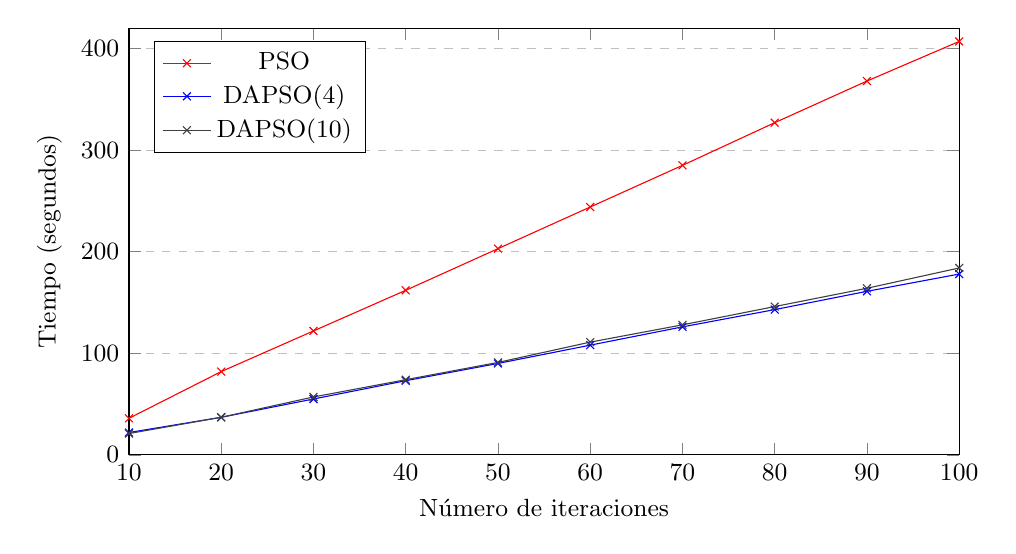
\begin{tikzpicture}[font=\small]
\begin{axis}[
    width=\textwidth,
    height=7cm,
    xlabel={Número de iteraciones},
    ylabel={Tiempo (segundos)},
    xmin=10, xmax=100,
    ymin=0, ymax=420,
    legend pos=north west,
    ymajorgrids=true,
    grid style=dashed,
]

\addplot[
    color=red,
    mark=x,
    ]
    coordinates {
    (10,36.0)(20,82.0)(30,122.0)(40,162.0)(50,203.0)(60,244.0)(70,285.0)(80,327.0)(90,368.0)(100,407.0)
    };

\addplot[
    color=blue,
    mark=x,
    ]
    coordinates {
    (10,22.0)(20,37.0)(30,55.0)(40,73.0)(50,90.0)(60,108.0)(70,126.0)(80,143.0)(90,161.0)(100,178.0)
    };
\addplot[
    color=darkgray,
    mark=x,
    ]
    coordinates {
    (10, 21.0)(20, 37.0)(30, 57.0)(40, 74.0)(50, 91.0)(60, 111.0)(70, 128.0)(80, 146.0)(90, 164.0)(100, 184.0)
    };
\legend{PSO, DAPSO(4), DAPSO(10)}
\end{axis}
\end{tikzpicture}
\end{minipage}%
\begin{minipage}[c]{.5\textwidth}
\resizebox{\textwidth}{!}{%
\raggedleft
    \begin{tabular}{c|ccc}
    \textbf{Nº de} & \multicolumn{3}{c}{\textbf{Tiempo de ejecución ($s$)}} \\ \cline{2-4} 
    \textbf{iters.} & \textit{PSO} & \textit{DAPSO(4)} & \textit{DAPSO(10)} \\ \hline
    10 & 36 & 22 & 21 \\
    20 & 82 & 37 & 37 \\
    30 & 122 & 55 & 57 \\
    40 & 162 & 73 & 74 \\
    50 & 203 & 90 & 91 \\
    60 & 244 & 108 & 111 \\
    70 & 285 & 126 & 128 \\
    80 & 327 & 143 & 146 \\
    90 & 368 & 161 & 164 \\
    100 & 407 & 178 & 184 \\
    \end{tabular}
}
\end{minipage}
    \caption{Comparativa en tiempo de entrenamiento del PSO secuencial y los distintos DAPSO en un problema de clasificación.}
    \label{fig:comp-tiempo-md}
\end{figure}

\begin{figure}[ht!]
\begin{minipage}[c]{.33\textwidth}
\resizebox{0.9\textwidth}{!}{%
    \renewcommand{\arraystretch}{2}
    \begin{tabular}{ll|x{0.8cm}|x{0.8cm}|}        
\multicolumn{2}{c}{}&   \multicolumn{2}{c}{Predicciones}\\
        \multicolumn{2}{c}{}&\multicolumn{1}{c}{\rotatebox[origin=c]{0}{Pos.}} & \multicolumn{1}{c}{\rotatebox[origin=c]{0}{Neg.}}\\
        \cline{3-4}
        \multirow{2}{*}{{\rotatebox[origin=c]{90}{Etiquetas}
        }} & 
        Pos. & 18 & 8  \\ \cline{3-4}
        &  Neg. & 14 & 74 \\ \cline{3-4}
    \end{tabular}
}
\end{minipage}%
\begin{minipage}[c]{.33\textwidth}
\resizebox{0.9\textwidth}{!}{%
    \centering
    \renewcommand{\arraystretch}{2}
    \begin{tabular}{ll|x{0.8cm}|x{0.8cm}|}        
\multicolumn{2}{c}{}&   \multicolumn{2}{c}{Predicciones}\\
        \multicolumn{2}{c}{}&\multicolumn{1}{c}{\rotatebox[origin=c]{0}{Pos.}} & \multicolumn{1}{c}{\rotatebox[origin=c]{0}{Neg.}}\\
        \cline{3-4}
        \multirow{2}{*}{{\rotatebox[origin=c]{90}{Etiquetas}
        }} & 
        Pos. & 23 & 3  \\ \cline{3-4}
        &  Neg. & 12 & 76 \\ \cline{3-4}
    \end{tabular}
}
\end{minipage}%
\begin{minipage}[c]{.33\textwidth}
\resizebox{0.9\textwidth}{!}{%
    \centering
    \renewcommand{\arraystretch}{2}
    \begin{tabular}{ll|x{0.8cm}|x{0.8cm}|}        
\multicolumn{2}{c}{}&   \multicolumn{2}{c}{Predicciones}\\
        \multicolumn{2}{c}{}&\multicolumn{1}{c}{\rotatebox[origin=c]{0}{Pos.}} & \multicolumn{1}{c}{\rotatebox[origin=c]{0}{Neg.}}\\
        \cline{3-4}
        \multirow{2}{*}{{\rotatebox[origin=c]{90}{Etiquetas}
        }} & 
        Pos. & 22 & 4  \\ \cline{3-4}
        &  Neg. & 9 & 79 \\ \cline{3-4}
    \end{tabular}
}
\end{minipage}
    \caption{Matrices de confusión de los clasificadores entrenados con 100 iteraciones por un algoritmo PSO, DAPSO con
    4 SuperRDDs y DAPSO con 10 SuperRDDs respectivamente.}
    \label{fig:conf-mat-prueba}
\end{figure}

\vspace{10pt}
Veamos ahora la comparativa en cuanto a la exactitud cuando se entrenaron con 100 iteraciones del algoritmo. Podemos 
observar las matrices de confusión de cada una de las redes en la figura \ref{fig:conf-mat-prueba}. Calculamos ahora las 
medidas mencionadas en el \autoref{chap:ann} para cada uno de los clasificadores a partir de esas matrices:

\begin{minipage}[c]{.33\textwidth}
\subsubsection*{Clasificador con algoritmo PSO}
\begin{itemize}
    \item \textit{Exactitud}: 0.8070
    \item \textit{Precisión}: 0.5625
    \item \textit{Sensibilidad}: 0.6923
    \item \textit{Puntuación $f_1$}: 0.3103
\end{itemize}
\end{minipage}%
\begin{minipage}[c]{.33\textwidth}
\subsubsection*{Clasificador con algoritmo DAPSO (4 SuperRDDs)}
\begin{itemize}
    \item \textit{Exactitud}: 0.8684
    \item \textit{Precisión}: 0.6571
    \item \textit{Sensibilidad}: 0.8846
    \item \textit{Puntuación $f_1$}: 0.3770
\end{itemize}
\end{minipage}%
\begin{minipage}[c]{.33\textwidth}
\subsubsection*{Clasificador con algoritmo DAPSO (10 SuperRDDs)}
\begin{itemize}
    \item \textit{Exactitud}: 0.8860
    \item \textit{Precisión}: 0.7097
    \item \textit{Sensibilidad}: 0.8846
    \item \textit{Puntuación $f_1$}: 0.3938
\end{itemize}
\end{minipage}%

\vspace{10pt}
Observamos cómo la versión distribuida proporciona mejores resultados en todas las medidas. Al tratarse de un modelo que
intenta predecir casos de cáncer, la mejora de sensibilidad de casi 0.2 al utilizar el algoritmo DAPSO es crucial. Para 
este problema, la mayor exploración del espacio de búsqueda lograda con la asíncronía, tal y como se describía en
\cite{dapso}, beneficia al modelo.

\vspace{10pt}
La segunda prueba nos servirá para validar los regresores implementados en la librería. Para ello, vamos a utilizar como
conjunto de datos los datos de consumo eléctrico de varios edificios de la Universidad de Granada. Para ello, vamos a
construir dos redes con 15 neuronas de entrada y 30 neuronas ocultas, y entrenaremos esas redes mediante un algoritmo PSO
y un algoritmo DAPSO respectivamente. Los parámetros de los algoritmos y las redes se encuentran especificados en la tabla
\ref{tab:conf-2}.

\vspace{10pt}
Un resumen visual de esta prueba puede encontrarse en la figura \ref{fig:comp-reg}. Una vez más, observamos que el 
algoritmo DAPSO tiene un tiempo de ejecución más de dos veces menor que su contraparte secuencial. La diferencia en este 
caso es más acusada (420 frente a 184 en el clasificador y 861 frente a 313 en el regresor), y se atribuye al aumento del
tamaño de la muestra (456 frente a 3000), mostrando de esta manera la mayor capacidad de escalabilidad que tiene el modelo
que utiliza un algoritmo sobre Spark. Esta capacidad aumentada la desarrollaremos más en la siguiente prueba.

\begin{table}[ht!]
    \centering
    \begin{tabular}{x{0.5\textwidth}x{0.3\textwidth}}
    \hline
    \textbf{Parámetro} & \textbf{Valor} \\
    \hline
    Tamaño de la muestra de entrenamiento & 3000 \\
    Iteraciones & 10, 20, 30, 40, 50, 60, 70, 80, 90, 100 \\
    Nº de neuronas en la capa de entrada & 15 \\
    Nº de neuronas en la capa oculta & 30 \\
    Nº de partículas PSO y DAPSO & 100 \\
    SuperRDDs & 4 \\
    Tamaño de los lotes & 10 \\
    Intervalo de posiciones & [-1,1] \\
    Intervalo de velocidades & [-0.6,0.6] (0.6$\times\text{pos max}$) \\
    $w$ & 1 \\
    $c_1$ & 0.8 \\
    $c_2$ & 0.2 \\
    \hline
    \end{tabular}
    \caption{Configuración de parámetros para la segunda prueba.}
    \label{tab:conf-2}
\end{table}

\begin{figure}[ht!]
\begin{minipage}[c]{.5\textwidth}
\raggedright
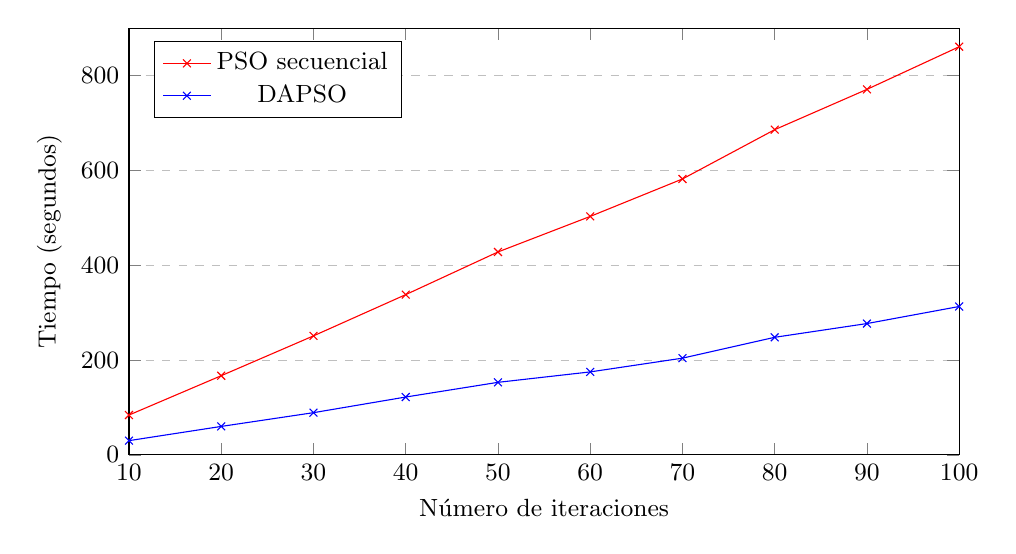
\begin{tikzpicture}[font=\small]
\begin{axis}[
    width=\textwidth,
    height=7cm,
    xlabel={Número de iteraciones},
    ylabel={Tiempo (segundos)},
    xmin=10, xmax=100,
    ymin=0, ymax=900,
    legend pos=north west,
    ymajorgrids=true,
    grid style=dashed,
]

\addplot[
    color=red,
    mark=x,
    ]
    coordinates {
    (10, 84.0)(20, 167.0)(30, 251.0)(40, 338.0)(50, 428.0)(60, 503.0)(70, 582.0)(80, 686.0)(90, 771.0)(100, 861.0)
    };
\addplot[
    color=blue,
    mark=x,
    ]
    coordinates {
    (10, 30.0)(20, 60.0)(30, 89.0)(40, 122.0)(50, 153.0)(60, 175.0)(70, 204.0)(80, 248.0)(90, 277.0)(100, 313.0)
    };
\legend{PSO secuencial, DAPSO}
\end{axis}
\end{tikzpicture}
\end{minipage}%
\begin{minipage}[c]{.5\textwidth}
\resizebox{\textwidth}{!}{%
\raggedleft
    \begin{tabular}{c|cc}
    \textbf{Nº de} & \multicolumn{2}{c}{\textbf{Tiempo ejecución ($s$)}} \\ \cline{2-3} 
    \textbf{iters} & \textit{PSO} & \textit{DAPSO} \\ \hline
10 & 84 & 30 \\
20 & 167 & 60 \\
30 & 251 & 89 \\
40 & 338 & 122 \\
50 & 428 & 153 \\
60 & 503 & 175 \\
70 & 582 & 204 \\
80 & 686 & 248 \\
90 & 771 & 277 \\
100 & 861 & 313 \\
    \end{tabular}
}
\end{minipage}
    \caption{Comparativa en tiempo de entrenamiento del PSO secuencial y el DAPSO para un problema de regresión.}
    \label{fig:comp-reg}
\end{figure}

\vspace{10pt}
En cuanto a la calidad de los resultados, podemos ver en la tabla \ref{tab:reg-mse} que en este caso el algoritmo DAPSO
se comporta peor que el secuencial. Estos difieren mucho de los obtenidos en 
\cite{iruela_ruiz_criado-ramón_pegalajar_capel_2024} (origen del conjunto de datos), pero lo podemos atribuir al tamaño
de la muestra escogido (3000) y el mínimo preprocesamiento de los datos. De cualquier manera, hemos comprobado el correcto
funcionamiento de los regresores en la librería.

\begin{table}[ht!]
    \centering
    \resizebox{\textwidth}{!}{%
\begin{tabular}{c|cccccccccc}
\textbf{Algoritmo de} & \multicolumn{10}{c}{\textbf{Iteraciones}} \\ \cline{2-11} 
\textbf{entrenamiento} & 10 & 20 & 30 & 40 & 50 & 60 & 70 & 80 & 90 & 100 \\ \hline
\textit{PSO secuencial} & 476.284 & 476.284 & 476.284 & 460.355 & 460.355 & 460.355 & 460.355 & 447.481 & 447.481 & 447.481
  \\
\textit{DAPSO} & 800.451 & 800.451 & 800.451 & 800.451 & 800.451 & 800.451 & 800.451 & 800.451 & 800.451 & 800.451
\end{tabular}
}
    \caption{Error cuadrático medio de los regresores para las distintas iteraciones.}
    \label{tab:reg-mse}
\end{table}

\vspace{10pt}
La tercera y última prueba a realizar viene a mostrar la capacidad de escalabilidad de la solución distribuida. Para ello 
usaremos un conjunto de datos de entrenamiento más grande, relacionado con los casos de COVID-19, y compararemos el 
tiempo de ejecución del algoritmo de entrenamiento frente a la cantidad de ejemplos utilizados en el proceso. Creamos 
para ello dos redes neuronales, que utilizarán una el PSO secuencial y la otra el DAPSO. Los parámetros para estos dos 
algoritmos serán los mismos que los utilizados para la prueba anterior, a excepción del número de partículas, que será 
ahora 50. En cuanto a las redes, ambas tendrán 23 neuronas en la capa de entrada y 46 en la de salida, y se entrenarán 
con 50 iteraciones. Un resumen de los parámetros lo podemos encontrar en la tabla \ref{tab:conf-3}.

\begin{table}[ht!]
    \centering
    \begin{tabular}{x{0.5\textwidth}x{0.3\textwidth}}
    \hline
    \textbf{Parámetro} & \textbf{Valor} \\
    \hline
    Tamaño de la muestra de entrenamiento & 500, 1000, 1500, 2000, 2500, 3000, 3500, 4000, 4500, 5000 \\
    Iteraciones & 50 \\
    Nº de neuronas en la capa de entrada & 23 \\
    Nº de neuronas en la capa oculta & 50 \\
    Nº de partículas PSO y DAPSO & 50 \\
    SuperRDDs & 4 \\
    Tamaño de los lotes & 10 \\
    Intervalo de posiciones & [-1,1] \\
    Intervalo de velocidades & [-0.6,0.6] (0.6$\times\text{pos max}$) \\
    $w$ & 0.721 ($\frac{1}{2\ln{2}}$) \\
    $c_1$, $c_2$ & 1.193 ($\frac 12+\ln{2}$) \\
    \hline
    \end{tabular}
    \caption{Configuración de parámetros para la tercera prueba.}
    \label{tab:conf-3}
\end{table}

\vspace{10pt}
El resultado de esta prueba se encuentra en la figura \ref{fig:comp-tiempo-dd}. Podemos apreciar claramente el beneficio 
que aporta el uso de algoritmos distribuidos y Spark en este caso. Conforme aumentamos el número de datos utilizados 
durante el entrenamiento, la diferencia en el tiempo de ejecución para el algoritmo secuencial y el paralelo aumenta a 
una gran velocidad. En particular, el algoritmo DAPSO es ya el doble de rápido (64 segundos frente a 32 segundos) cuando
el tamaño de la muestra es de únicamente 500 ejemplos, llegando a más del triple (824 segundos frente a 264 segundos) 
cuando la muestra contiene 5000 ejemplos.

\begin{figure}[ht!]
\begin{minipage}[c]{.5\textwidth}
\raggedright
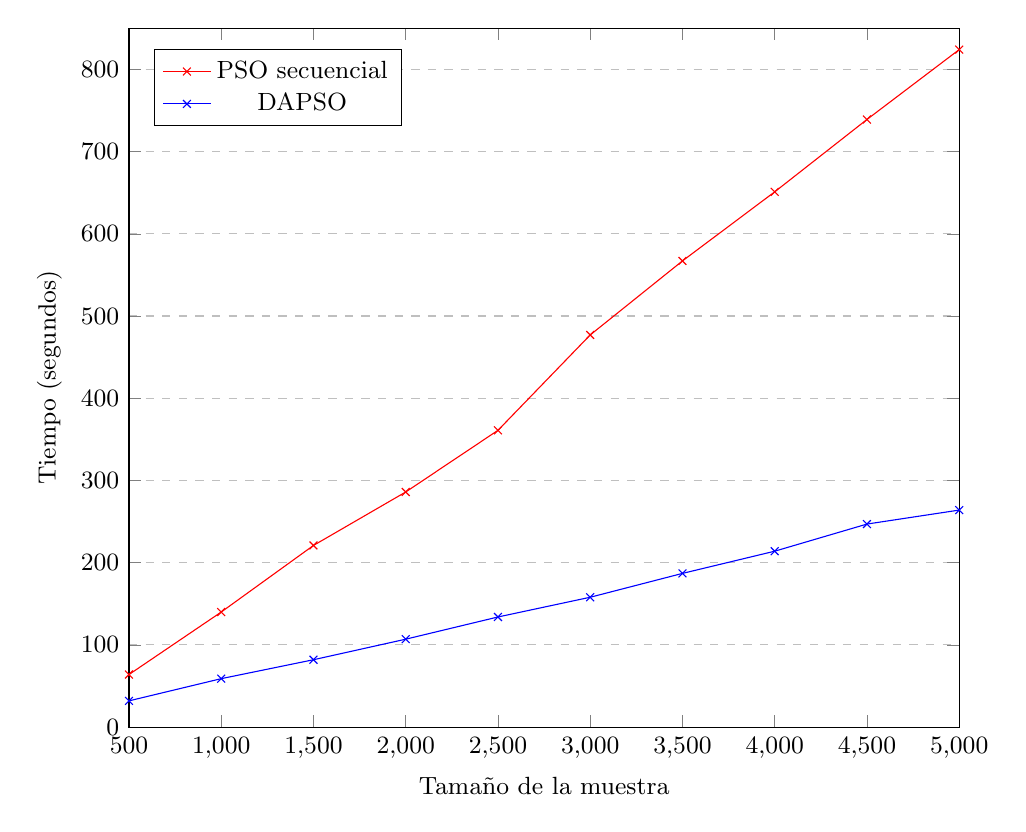
\begin{tikzpicture}[font=\small]
\begin{axis}[
    width=\textwidth,
    xlabel={Tamaño de la muestra},
    ylabel={Tiempo (segundos)},
    xmin=500, xmax=5000,
    ymin=0, ymax=850,
    legend pos=north west,
    ymajorgrids=true,
    grid style=dashed,
]

\addplot[
    color=red,
    mark=x,
    ]
    coordinates {
    (500, 64.0)(1000, 140.0)(1500, 221.0)(2000, 286.0)(2500, 361.0)(3000, 477.0)(3500, 567.0)(4000, 651.0)(4500, 739.0)(5000, 824.0)
    };
\addplot[
    color=blue,
    mark=x,
    ]
    coordinates {
    (500, 32.0)(1000, 59.0)(1500, 82.0)(2000, 107.0)(2500, 134.0)(3000, 158.0)(3500, 187.0)(4000, 214.0)(4500, 247.0)(5000, 264.0)

    };
\legend{PSO secuencial, DAPSO}
\end{axis}
\end{tikzpicture}
\end{minipage}%
\begin{minipage}[c]{.5\textwidth}
\resizebox{\textwidth}{!}{%
\raggedleft
    \begin{tabular}{c|cc}
    \textbf{Tamaño de} & \multicolumn{2}{c}{\textbf{Tiempo ejecución ($s$)}} \\ \cline{2-3} 
    \textbf{la muestra} & \textit{PSO} & \textit{DAPSO} \\ \hline
    500 & 64 & 32 \\
    1000 & 140 & 59 \\
    1500 & 221 & 82 \\
    2000 & 286 & 107 \\
    2500 & 361 & 134 \\
    3000 & 477 & 158 \\
    3500 & 567 & 187 \\
    4000 & 651 & 214 \\
    4500 & 739 & 247 \\
    5000 & 824 & 264 \\
    \end{tabular}
}
\end{minipage}
    \caption{Comparativa en tiempo de entrenamiento del PSO secuencial y el DAPSO para diferentes muestras de entrenamiento.}
    \label{fig:comp-tiempo-dd}
\end{figure}

\vspace{10pt}
En definitiva, hemos comprobado el correcto funcionamiento, mediante estas tres pruebas, de la librería implementada en el
proyecto. También hemos comprobado la mejora sustancial en tiempos de ejecución del algoritmo DAPSO, mostrando también sus
altas capacidades de escalabilidad al aumentar el tamaño de la muestra con la que se trabaja, proporcionando así una 
solución al problema presentado en la introducción.

\section{Intérprete}

Vamos a mostrar el analizador léxico y el explorador del intérprete de SSDL creado. A partir de unas piezas de código,
mostraremos la lista de \textit{tokens} generada y el árbol de sintaxis abstracta generado.

\vspace{10pt}
Comenzamos con la descripción de un algoritmo DAPSO. La pieza de código que lo genera es la siguiente
(figura \ref{fig:dapso-ssdl}):

\begin{figure}[ht!]
    \centering
    \StartLineAt{1}
    \lstinputlisting[language=Pascal]{code/dapso.ssdl}
    \caption{Código en SSDL para la configuración de un algoritmo DAPSO}
    \label{fig:dapso-ssdl}
\end{figure}

El analizador léxico del lenguaje genera, para esa secuencia, los siguientes \textit{tokens}:
\vspace{10pt}
\begin{lstlisting}[numbers=none]
[@0,29:33='begin',<'begin'>,2:0]
[@1,35:39='dapso',<OBJECT>,2:6]
[@2,40:40=':',<':'>,2:11]
[@3,42:46='DAPSO',<ID>,2:13]
[@4,52:54='set',<'set'>,3:4]
[@5,56:64='particles',<'particles'>,3:8]
[@6,66:67='50',<INT>,3:18]
[@7,73:75='set',<'set'>,4:4]
[@8,77:85='pos_bound',<'pos_bound'>,4:8]
[@9,87:89='2.0',<FLOAT>,4:18]
[@10,95:97='set',<'set'>,5:4]
[@11,99:108='batch_size',<'batch_size'>,5:8]
[@12,110:111='10',<INT>,5:19]
[@13,113:115='end',<'end'>,6:0]
[@14,116:115='<EOF>',<EOF>,6:3]
\end{lstlisting}

Podemos ver que los comentarios, al no generar ninguna sentencia, son ignorados por el analizador, simplificando 
en adelante el árbol de sintaxis abstracta. Veamos ahora el árbol de sintaxis abstracta o AST del programa (figura 
\ref{fig:dapso-ast}):

\begin{figure}[ht!]
    \centering
    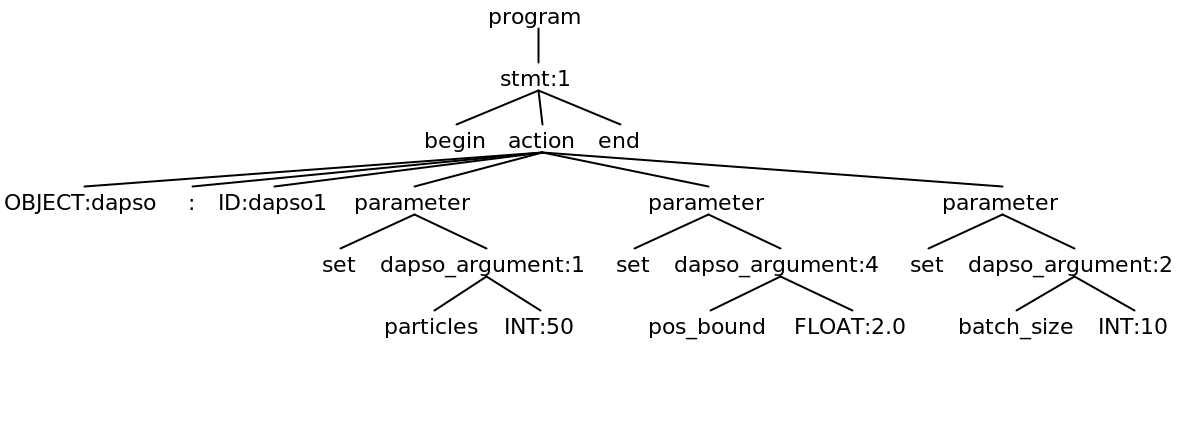
\includegraphics[width=1\linewidth]{img/dapso_ast.png}
    \caption{AST para la configuración de un algoritmo DAPSO.}
    \label{fig:dapso-ast}
\end{figure}

\vspace{10pt}
El código que generaría el intérprete a partir del AST, usando la librería implementada sería el de la figura 
\ref{fig:dapso-ssdl-scala}.

\vspace{10pt}
\begin{figure}[ht!]
    \StartLineAt{1}
    \begin{lstlisting}[language=Scala]
val dapso1 = new DAPSO(50, 2.0, batchSize = 10)
    \end{lstlisting}
    \caption{Código en Scala equivalente a la especificación en SSDL de la figura \ref{fig:dapso-ast}.}
    \label{fig:dapso-ssdl-scala}
\end{figure}

Veamos ahora una pieza de código más compleja. Supongamos que, después del código mostrado anteriormente, encontramos el 
siguiente código (figura \ref{fig:ann-ssdl}):

\begin{figure}[ht!]
    \centering
    \StartLineAt{7}
    \lstinputlisting[language=Pascal]{code/ann.ssdl}
    \caption{Código en SSDL para la configuración, entrenamiento y exportación de datos de una red neuronal.}
    \label{fig:ann-ssdl}
\end{figure}

El analizador léxico creado extrae la siguiente lista de \textit{tokens}:
\vspace{10pt}
\begin{lstlisting}[numbers=none]
[@0,36:40='begin',<'begin'>,2:0]
[@1,42:44='ann',<OBJECT>,2:6]
[@2,45:45=':',<':'>,2:9]
[@3,47:51='clas1',<ID>,2:11]
[@4,57:59='set',<'set'>,3:4]
[@5,61:64='type',<'type'>,3:8]
[@6,66:75='classifier',<NET_TYPE>,3:13]
[@7,81:83='set',<'set'>,4:4]
[@8,85:91='neurons',<'neurons'>,4:8]
[@9,93:93='[',<'['>,4:16]
[@10,94:95='50',<INT>,4:17]
[@11,96:96=',',<','>,4:19]
[@12,97:99='200',<INT>,4:20]
[@13,100:100=']',<']'>,4:23]
[@14,106:108='set',<'set'>,5:4]
[@15,110:113='data',<'data'>,5:8]
[@16,115:115='[',<'['>,5:13]
[@17,116:135='"covid_training.csv"',<FILE>,5:14]
[@18,136:136=',',<','>,5:34]
[@19,137:152='"covid_test.csv"',<FILE>,5:35]
[@20,153:153=']',<']'>,5:51]
[@21,159:161='set',<'set'>,6:4]
[@22,163:171='algorithm',<'algorithm'>,6:8]
[@23,173:177='DAPSO',<ID>,6:18]
[@24,179:181='end',<'end'>,7:0]
[@25,203:205='fit',<'fit'>,9:0]
[@26,207:211='clas1',<ID>,9:4]
[@27,213:215='100',<INT>,9:10]
[@28,217:219='out',<'out'>,10:0]
[@29,221:225='clas1',<ID>,10:4]
[@30,227:248='"clasificador_100.csv"',<FILE>,10:10]
[@31,249:248='<EOF>',<EOF>,10:32]
\end{lstlisting}

Generando a partir de ella el explorador el AST siguiente (figura \ref{fig:ann-ast}):

\begin{figure}[ht!]
    \centering
    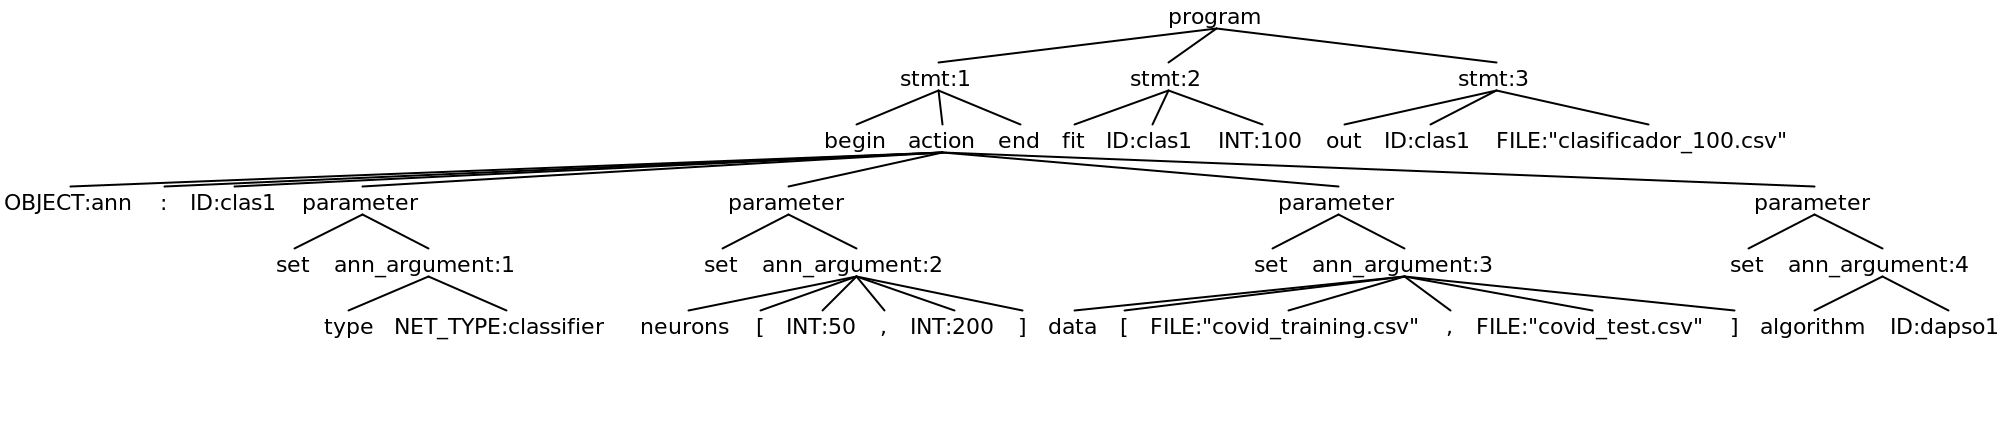
\includegraphics[width=1\linewidth]{img/ann_ast.png}
    \caption{AST para la configuración, entrenamiento y exportación de pesos de una red neuronal.}
    \label{fig:ann-ast}
\end{figure}

Unificando este AST con el anterior, obtenemos un programa completo que especifica los parámetros de un algoritmo DAPSO,
configura una red neuronal con ese algoritmo, la entrena y exporta los pesos obtenidos de ese entrenamiento. El código que
el intérprete escribiría a partir del árbol aparece en la figura \ref{fig:ssdl-scala}.

\vspace{10pt}
\begin{figure}[ht!]
    \centering
    \StartLineAt{1}
    \begin{lstlisting}[language=Scala]
val dapso1 = new DAPSO(50, 2.0, batchSize = 10)

val clas1 = new Classifier(50,200)
clas1.setTrainingData("covid_training.csv", Int.MaxValue)
clas1.setTestData("covid_test.csv", Int.MaxValue)
clas1.setTrainer(dapso1)

clas1.fit(100)
clas1.writeWeights("clasificador_100.csv")
    \end{lstlisting}
    \caption{Código en Scala equivalente a la especificación en SSDL de las figuras \ref{fig:dapso-ast} y \ref{fig:ann-ast}.}
    \label{fig:ssdl-scala}
\end{figure}

\endinput
%--------------------------------------------------------------------
% FIN DEL CAPÍTULO. 
%--------------------------------------------------------------------
